\documentclass[12pt, letterpaper]{article}

\usepackage{graphicx}
\usepackage{parskip} % Disabling paragraph index as it does not fit maths
\usepackage{amssymb} % Used to show sets of sumbers, like the real numbers
\usepackage{hyperref} % Usable menu and references

\graphicspath{{images}}

\title{Algebra II}
\author{Arkadiusz Naks}
\date{2023}

\begin{document}

\begin{titlepage}
  \begin{center}
    \makeatletter
    \vspace*{1cm}
    \Huge
    \textbf{\@title}

    \vspace{0.5cm}
    \Large
    Lecture notes from Algebra 2 module at Durham University

    \vspace{1.5cm}

    \textbf{\@author}

    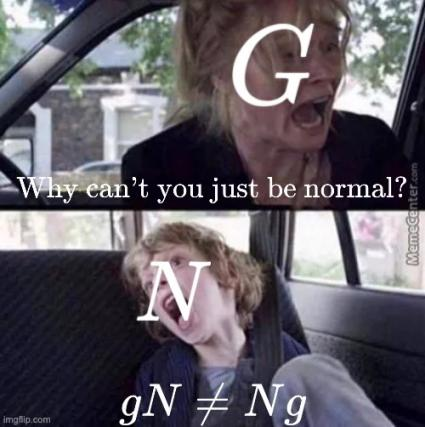
\includegraphics[scale=0.55]{algebra.png}
    \vfill

    \vspace{0.8cm}

    \small
    Based on my understanding of lectures and notes of Prof Anrew Jay Lobb,
    based on notes by Prof Dirk Shutz\\
    \@date{}
  \end{center}
\end{titlepage}

\tableofcontents
\newpage

\begin{section}{Important Definisions}
  A place for short and important definisions

  \textsc{Definision} (Cardinality) \textit{Number of elements in a set or any
    more complex structure}

  \textsc{Definision} (Disjoint) \textit{Two sets with no common elements}

  \textsc{Definision} (Commutativity) \textit{}

  \textsc{Definision} (Closure) \textit{A set G is closed under an operation
    \(\bullet\) if \newline \(\forall a, b \in G \; a \bullet b \in G\).}

  \textsc{Definision} (Associativity) \textit{An operation \(\bullet\) is called
    \textbf{associative} for three elements a,b,c if
    \(a \bullet (b \bullet c) = (a \bullet b) \bullet c\).}

  \textsc{Definision} (Identity) \textit{An element i in a set S is called \textbf{the identity}
    for an operation \(\bullet\) if \(i \bullet a = a \bullet i = a \; \forall a \in S\).}

  \textsc{Definision} (Inverse) \textit{An element a is called \textbf{invertable} under an
    operation \(\bullet\) if \(\exists\) b s.t. \(a \bullet b = b \bullet a = i\) where
    i is the identity.}

\end{section}

\begin{section}{Groups}

  \begin{subsection}{Group basics}

    \begin{subsubsection}{Definisions}

      A \textbf{group} is a set G and an operation \(\bullet\). It is denoted as
      \((G, \bullet)\). A \textbf{group} has to
      \begin{itemize}
        \item Be \textbf{closed}
        \item Be \textbf{associative} \(\forall a,b,c \in G\)
        \item Contain \textbf{identity}, usually denoted as \(i \in G\)
        \item All \(g \in G\) must contain an \textbf{inverse}, denoted as \(g^{-1}\)
      \end{itemize}
      A \textbf{group} is called \textbf{abelian} if \(\bullet\) is \textbf{commutative}
      \(\forall g, h \in G\).

      For simplisitys sake a \textbf{group} \((G, \bullet)\) will be denoted as just G
      if the operation is obvious.

      A \textbf{group} \((G, \bullet)\) is called \textbf{finite} if the set G is finite.
      In such case the order of G is denoted at \(\#G\) and is the size of the set G.

    \end{subsubsection}

    \begin{subsubsection}{Centre}

      Group \textbf{centre}, denoted as \(Z(G)\), is defined to be all
      \(g \in G\) s.t.\ \(hgh^{-1} = g \; \forall h \in G\). In words centre is
      a set of all \(g \in G\) which \textbf{commute} with all other elemets in G.

      Some properties of the centre \:
      \begin{itemize}
        \item Z(G) is a \textbf{normal} subgroup of G
        \item It is the union of all conjugacy classes of size 1
        \item \(Z(G) = G \iff G\) is \textbf{abelian}
        \item If G acts on itself by conjugation then for any \(g \ in G\)
              \(Z(G) \subset G_{g}\)
        \item For a prime p a group G of order \(p^{r}\) is
              \textbf{non-trivial}
      \end{itemize}

    \end{subsubsection}

    \begin{subsubsection}{Conjugation and Commutation}

      Two elements \(g, g'\) where \(g \neq g'\) are called \textbf{conjugate} in G
      if \(\exists h \in G \) s.t. \(hgh^{-1} = g'\).

      A \textbf{conjugacy class} of an element in G is defined as
      \(ccl_{G}(g) = {hgh^{-1} | \forall h \in G}\).

      If all conjugacy classes are of size 1, G is \textbf{abelian}.

      For \(g \in G\) to \textbf{commute} with \(h \in G\) it means \(hg = gh\)
      or \(hgh^{-1} = g\), or in words g conjugates to itself with h.

    \end{subsubsection}

    \begin{subsubsection}{Order}

      The \textbf{order} of an element \(g \in G\) is defined as the smallest
      integer r s.t. \(g^{r} = e\), where e is the \textbf{identity} in G.
      If such r does not exists, the order of g is \(\infty\).
      This is denoted as \(ord(g)\).

    \end{subsubsection}

    \begin{subsubsection}{Generated Groups}

      Any group that can be represented as powers of some
      \(\{ g_{1}, \dots , g_{r} \}\) is said to be \textbf{finitely generated}.

      Any \textbf{abelian} group can be writen as a \textbf{guotient} group
      \(G \approx \mathbb{Z}^{n} / K\) where \(K \leq \mathbb{Z}^{n}\). K is
      called a \textbf{relation subgroup} of G and any \(a \in K\) is a
      \textbf{relation}. If there \(a \neq 0 \; \forall a \in K\) G is called
      \textbf{free abelian group of rank n}. \\
      Every subgroup \(H \leq \mathbb{Z}^{n}\) is \textbf{free} with
      \(rank \leq n\). H is generated by \(r \leq n\) elements. These elements
      can be represented as a \textbf{relation matrix} denoted as \(A(H)\).
      This can be simply denoted as A.  \\
      Any matrix with \(A \in Mat_{m \times z}(\mathbb{Z})\) can be transformed
      into a diagonal matrix \(\tilde{A} \in Mat_{m \times n}(\mathbb{Z})\) with
      elementary operations. In this config
      \(\tilde{a}_{1, 1} | \tilde{a}_{2, 2} | \dots | \tilde{a}_{m, m}\).

      This results in the long named \textbf{Fundamental Theorem of Finitely
        Generated Abelian Groups} which says all G finitely generated and abelian
      groups are isomorphic to \(\mathbb{Z} / d_{1} \times \cdots \times
      \mathbb{Z} / d_{k} \times \mathbb{Z}^{r}\) with \(r, k \geq 0\) and all
      \(d_{i} \geq 1\). If \(d_{1} | d_{2} | \dots | d_{k}\) and \(d_{1} > 1\)
      is unique. The number r is the rank of G and ds are called \textbf{torsion
        invarsions}. Some properties of such groups
      \begin{itemize}
        \item \(r = 0 \iff |G| \neq \infty\)
        \item \(r = k = 0\) G is trival group
        \item 1 never occures in \textbf{torsion invarion}
      \end{itemize}

      \textbf{Cyclic}
      If a group can be generated by one element, \(G = \langle g \rangle\),
      it is called a \textbf{cyclc group}.

      \emph{Any \textbf{cyclic} groups are always \textbf{abelian}} \\
      \emph{If \#G is prime G is a \textbf{cyclic}}

    \end{subsubsection}

    \begin{subsubsection}{The Dihedral Groups}

      This groups are denoted as \(D_{n}\) for \(n \geq 3\) and they represent
      all rotations and reflectios of an n-gon. The group size is always \(2n\).
      With rotations being represented as r and reflectios as s this group can be
      generated by \(\langle r, s \rangle\) where \(r^{n} = e, s^{2} = e, srs^{-1} = r^{-1}\).
      The e is the identity.

      Moreever the rotation elements form a \textbf{normal cyclic} subgroup of \(D_{n}\),
      \(\langle r \rangle\).

    \end{subsubsection}

    \begin{subsubsection}{Some Group Rules}

      \textbf{Cauchy} \\
      Any group G of order 2p with p odd prime, then it is either \textbf{cyclic}
      or \textbf{dihedral}.
      For a finite group G and a prime p s.t.\ \(p | |G|\) then there is a
      subgroup of G of order p. \\

      \textbf{Sylow} \\
      Following from \textbf{Cauchy} any group of order \(p^{r}m\) with p prime
      and \(\gcd(p, m) = 1\) has a subgroup of order
      \(p^{1} \; \forall i \in [1, r]\).

      \emph{Any groups of order \(p^{2}\) with p prime are \textbf{abelian}} \\
      Moreever \(G \approx \mathbb{Z} / p\) or
      \(G \approx \mathbb{Z} / p \times \mathbb{Z} / p\).

    \end{subsubsection}

  \end{subsection}

  \begin{subsection}{Permutation groups}

    Permutation group \((G, \bullet)\), denoted as \(S_{n}\), is a set
    \(G = \{ 1, 2 \dots n \}\) and \(\bullet\) a bijection.
    For a permutation group \(\#S_{n} = n!\). \\

    \begin{subsubsection}{Cycles}

      Two cycles are called \textbf{disjoinet} if their members do not intersect.
      Any \(g \in S_{n}\) can be writen as a product of \textbf{disjoinet}
      cycles, and by sorting the lenght of these cycles \textbf{cycle shape} can
      be optained.

      For a cyce For any \(g \in S_{n}\) and
      \(h = (i_{1}, i_{2}, \dots . i_{k})\)
      \(ghg^{-1} = (g(i_{1}), g(i_{1}), \dots , g(i_{k}))\). \\
      This means the conjugacy class \(ccl_{S_{n}}(x)\) is all permutations of
      the same cycle shape as x.

      A cycle of length 2 is called a \textbf{transposition}. Any
      \textbf{conjugate} of a \textbf{transposition} is also a
      \textbf{transposition}. \\

      Any \(g \in S_{n}\) can be described as a product of
      \textbf{transpositions}.
      This factorisation has a pairity (odd or even). \\

      \emph{How many k-cycles in \(S_{n}\) \[\frac{n!}{k(n-k+1)!}\]}

    \end{subsubsection}

    \begin{subsubsection}{Altering Group}

      A sign of \(g \in S_{n}\) is 1 if its even, -1 if its odd. \\
      The \textbf{alternating group} \(A_{n}\) is defined to be the subgroup of
      all the even permuations in \(S_{n}\). This subgroup is \textbf{normal} and
      can always be generated by 3-cycles.

      \emph{\(\forall x \in A_{n} \; ccl_{A_{n}}(x) \subset ccl_{S_{n}}(x)\)} \\
      More specifically if x \textbf{commutes} with some odd permutations then
      they are equal, else
      \(ccl_{S_{n}}(x) = ccl_{A_{n}} \cup ccl_{A_{n}}((1 \; 2) x (1 \; 2))\).

    \end{subsubsection}

  \end{subsection}

  \begin{subsection}{Subgroups}

    \begin{subsubsection}{Basics}

      For a given \textbf{group} \((G, \bullet)\) \((H, \bullet)\) is a \textbf{subgroup}
      if \(H \subset G\), \(H \neq \emptyset\), H is \textbf{closed} under \(\bullet\)
      and \(\forall g \in H \; \exists g^{-1}\) (\textbf{inverses}). \textbf{Identity}
      is guarenteed by \textbf{inverses} and \textbf{closure} and \textbf{associativity}
      is inhereted from \(G, \bullet\). This is denoted as \((H, \bullet) < (G, \bullet)\) \\
      A \textbf{subgroup} is called \textbf{proper} if \(H \neq \{{} e \}{}\) and
      \(H \neq G\).

      \emph{For a \textbf{finite group} \((G, \bullet)\) every \textbf{subgroup}
        \(H < G\) follows \(\#H|\#G\).}

    \end{subsubsection}

    \begin{subsubsection}{Normal}

      A \textbf{subgroup} is called \textbf{normal} if the \textbf{left} and
      \textbf{right cosets} are identical for any \(g \in G\), \(gH = Hg\).
      This is denoted as \(H \triangleleft G\). Alternatively is can be denoted as
      \[ghg^{-1} \in H \;\; \forall g \in G \; \forall h \in H \;\;
        or \;\; gHg^{-1} \subset H \;\; \forall g \in G\]

      H is a normal \textbf{subgroup} of G iff H is a union of \textbf{conjugacy classe}
      of G.

      Normal subgroups play an analogous role to ideals in groups.

    \end{subsubsection}

    \begin{subsubsection}{Quotient Group}

      For N a \textbf{normal} subgroup of \((G, \cdot)\), then a quotient group
      \((G_{N}, \cdot_{N})\) of G with respect to N is induced from G on the set
      of cosets \(\{ gN | g \in G \}\). Its operation, \(\cdot_{N}\), is defined as
      \(g_{1}N \cdot_{N} g_{2}N = (g_{1} \cdot g_{2})N\) and therefor inverses are
      \((gN)^{-1} = (g^{-1})N\).

    \end{subsubsection}

    \begin{subsubsection}{Generators}

      A \textbf{subgroup} H of G is said to be \textbf{generated} by \(g \in G\),
      denoted \(\langle g \rangle\), if \(H = \{ g^{n} \; | \; \forall n \in \mathbb{Z} \}\). \\
      More generally for every subset of G a subgroup generated by all elements
      of this subset can be defined (this idea is very similar to baisis for a
      vectorspace).

    \end{subsubsection}

  \end{subsection}

  \begin{subsection}{Cosets}

    \textbf{Left coset} of g with respect to H in G is defined for \(H < G\)
    and \(g \in G\) as \(g \bullet H = \{{} g \bullet h \; | \; \forall h \in H \}{}\).
    A \textbf{left coset} can be construct for any \(g \in G\). \\
    Similarly a \textbf{right coset} of g is defined as
    \(H \bullet g = \{{} h \bullet g \; | \; \forall h \in H \}{}\). \\
    Properies of different \textbf{cosets} with respect to H in G:
    \begin{itemize}
      \item All \textbf{same cosets} have the same \textbf{cardinality}
      \item Two \textbf{same cosets} are either \textbf{disjoint} or \textbf{identical}
    \end{itemize}

  \end{subsection}

  \begin{subsection}{Group Homomorphisms and Isomorphisms}

    \begin{subsubsection}{Some Isomorphisms}

      \begin{itemize}
        \item \(A_{3}, C_{3}\)
        \item \(S_{2}, C_{2}\)
        \item \(S_{3}, D_{3}\)
        \item \(D_{2k}, D_{k} \times \mathbb{Z} / 2\)
        \item \(\mathbb{Z} / mn, \mathbb{Z} / m \times \mathbb{Z} / n\) if \(\gcd(m, n) = 1\)
        \item \(S_{4}\) and rotational symetries of a cube in \(\mathbb{R}^{3}\)
      \end{itemize}

      For p prime any group of order p is isomorphic to \((\mathbb{Z} / p, +)\). \\
      Each \textbf{cyclic} group of order n is isomorphic to \(\mathbb{Z} \ n, +\)
      and this follows with \(n \to \infty\).

      In fact each group \((G, \cdot)\) is isomorphic to a subgroup of some
      permuation \(S_{p}\).

    \end{subsubsection}

    \begin{subsubsection}{Homomorphism}

      The only requirement for a homomorphism is for groups \((G_{1}, \cdot_{1}),
      (G_{2}, \cdot_{2})\) and \(g_{1}, g_{2} \in G_{1}\):
      \[\varphi(g_{1} \cdot_{1} g_{2}) = \varphi(g_{1}) \cdot_{2} \varphi(g_{2}).\]

      If this is true for all the generators of a group it is true for the whole
      group.

    \end{subsubsection}

    \begin{subsubsection}{Isomorphism}

      For G and H to be isomorphic, denoted as \(G \simeq H\), requires them
      to have a  homomorphism \(\varphi\) which is also \textbf{bijective}.

      An isomorphism preserves:
      \begin{itemize}
        \item Order of a group
        \item Orders af all elements
        \item Size of the center (??)
        \item Abelian or not
        \item Size of normal subgroups
      \end{itemize}

    \end{subsubsection}

    \begin{subsubsection}{Image and Kernal}

      A kernal of a homomorphism \(\varphi : G \to H\) is a set of all \(g \in G\)
      which go to \(e \in H\), \(\ker(\varphi) = \{ g \in G | \varphi(g) = e \}\).
      The kernal is a normal subgroup of G.

      Meanwhile the image is all \(h \in H\) which can be obtained by \(\varphi\),
      \(im(\varphi) = \{ \varphi(g) | g \in G \}\).
      The image is a subgroup of H.

    \end{subsubsection}

    \begin{subsubsection}{First Isomorphic Theorem for Groups (and others)}

      Similarly as for rings, \[G / \ker(\varphi) \simeq im(\varphi).\]

      This shows any homomorphism which is bijective is an isomorphism as
      \(bijective \iff \ker{\varphi} = \emptyset\).

      For H and K subgroups of G s.t.
      \begin{itemize}
        \item \(H \cdot K = G\)
        \item \(H \cap K = \{ e \}\)
        \item \(hk = kh \; \forall h \in H \forall k \in K\)
      \end{itemize}
      Then \(G \simeq H \times K\).

    \end{subsubsection}

  \end{subsection}

  \begin{subsection}{Group Products and Actions}

    \begin{subsubsection}{Product}

      Cartesian product of two groups \(G \times H\) is also a group. \\
      This is defined as \(G \times H = \{ (g, h) | \forall g \in G \forall h \in H \}\)

    \end{subsubsection}

    \begin{subsubsection}{Action}

      An action of a group G on a set \(X \neq \emptyset\) is a homomorphism.
      The homomorphism is \(\varphi : G \to S_{X}\), the result is a permuation
      of X. The action is applied by \(\varphi(g)(x)\) or simply \(g(x)\).

      A group \((G, \cdot)\) can act on itself, meaing \(X = G\).  There are two
      ways such action can be implemented
      \begin{enumerate}
        \item by left translation \(g \in G\) acts on \(h \in G\) by
              \(g(h) = g \cdot h\) \\
              Orbit of any h is the whole set G \\
              Stabiliser of each h is \(\{ e \}\)
        \item by conjugation \(g \in G\) act on \(h \in G\) by
              \(g(h) = ghg^{-1}\)
      \end{enumerate}

    \end{subsubsection}

  \end{subsection}

  \begin{subsection}{Orbits and Stabilisers}

    For a group action \(\varphi : G \to S_{X}\) then for every \(x \in X\) \\
    \textbf{G-orbit} is \(G(x) := \{ \varphi(g)(x) | g \in G \}\) \\
    \textbf{Stabiliser of G} is \(G_{x} := \{ g \in G | \varphi(g)(x) = x \}\) \\

    For any group action of G on X there exists a \textbf{bijection} for any
    \(x \in X\) \(\beta : G(x) \to\) \{left cosets of \(G_{x} \in G\)\} taking
    \(g(x)\) to \(gG_{x}\). \\
    This means \(|G(x)| \times |G_{x}| = |G|\) if G and X are finite. Although
    this still works for infinite, but not very useful. This also implies
    \(|G(x)|\) divides \(|G|\).

    \begin{subsubsection}{Orbits}

      \begin{itemize}
        \item Each orbit \(G(x)\) is a non emptyset subset of X
        \item Union of all orbits is whole set X
        \item Each orbit is either the same or disjoint from all others
      \end{itemize}

      An orbit under conjugation of \(g \in G\) is the \textbf{conjugacy class}
      of g, \(G(x) = ccl_{G}(g)\) where the action is conjugation.

      If \(x \in G_{y}\) then \(G_{x} = hG_{y}h^{-1}\) for some \(h \in G\).

    \end{subsubsection}

    \begin{subsubsection}{Stabilisers}

      Any stabiliser \(G_{x}\) is a subgroup of G.

    \end{subsubsection}

  \end{subsection}

\end{section}

\begin{section}{Rings}

  This section will touch on \textbf{rings} as well as other number structures
  such as \textbf{fields}.

  \begin{subsection}{Ring Definision}

    A \textbf{ring} is a set together with two operation, denoted as \(+, \cdot\).
    A group made by \(R, +\) has to be \textbf{abelian}. For \(\cdot\) R has to
    \begin{itemize}
      \item contain \textbf{identity}
      \item be \textbf{associative}
      \item be \textbf{distributive} together with \(+\), meaning
            for \(x, y, z \in R \; x \cdot (y + z) = x \cdot y + x \cdot z\) and
            for \(x, y, z \in R \; (y + z) \cdot x = y \cdot x + z \cdot x\)
      \item \textbf{closure}
    \end{itemize}

    Identities for \(+\) and \(\cdot\) are usually represented as 0 and 1.

    For a ring \(a \cdot b\) can be writen as \(ab\).

    By \textbf{Chinese Remainder Theorem},
    \(\mathbb{Z}/(n_{1}n_{2} \dots n_{m}) \approxeq \mathbb{Z}/n_{1} \times
    \mathbb{Z}/n_{2} \times \dots \times \mathbb{Z}/n_{m}\) for
    \(\gcd(n_{1}, n_{2}, \dots , n_{m}) = 1\).

  \end{subsection}

  \begin{subsection}{Subring}

    A \textbf{subring} is a smaller ring with the same operations as its
    parrent ring. \textbf{Subring} is required to contain both \textbf{identites}.
    It also has to be \textbf{closed} under both operation and \textbf{inverses}
    of \(+\) have to exist in it.

    \emph{The ring itself is always its own subring}

  \end{subsection}

  \begin{subsection}{Fields}

    A \textbf{field} is a stricter version of a \textbf{ring}. For R to be a
    \textbf{field} R has to be \textbf{ring} as well as
    \begin{itemize}
      \item \textbf{commutative} for \(\cdot\)
            (already commutative for \(+\) to be a ring)
      \item \(1 \neq 0 \in R\)
      \item \(\forall a \in R \; a \neq 0 \; \exists b \; s.t. \; a \cdot b = 1\)
            meaning all nonzero elements have inverses for \(\cdot\)
    \end{itemize}

    If F a \textbf{field} then for \(a, b \in F \; ab = 0 \iff a = 0 \; or \; b = 0\).

    \(\mathbb{Z}/n\) is a field \(\iff n\) is prime

    \begin{subsubsection}{Polynomial Fields}

      A polynomial field is defined as
      \(f(x) = a_{0}x^{0} + a_{1}x^{1} + \dots + a_{n}x^{n} \in F[x]\) \\
      \(\deg(f)\) is the biggest power of x in \(f(x)\). If \(f(x) = 0\) then
      \(\deg(f) = -\inf\) \\
      Then for \(f(x), g(x) \in F[x]\)
      \begin{itemize}
        \item \(\deg{fg} = \deg(f) + \deg{g}\)
        \item \(\deg(f + g) \leq \max\{ \deg(f), \deg(g) \}\)
        \item if \(\deg(f) \neq \deg(g)\) then \(\deg(f + g) = \max\{ \deg(f), \deg(g) \}\)
      \end{itemize}

      For \(f(x), g(x) \in F[x]\) with \(g(x) \neq 0\) then \(\exists q(x), r(x) \in F[x]\)
      with \(\deg(r) < \deg(g)\) s.t. \(f(x) = q(x)g(x) + r(x)\).

      For F a field and \(f(x) \in F[x]\) irreducable. Then \(F[x]/(f(x))\) is a field
      and a \textbf{vectorspace} over F with a basis \(1, x, \dots , x^{n - 1}\)
      with \(n = \deg(f(x))\).

    \end{subsubsection}

    \begin{subsubsection}{Special}

      For any prime \(p \in \mathbb{Z}\) and \(n \in \mathbb{N}\)
      \(\exists f(x) \in (\mathbb{Z} / p)[x]\) where \(\deg(f(x)) = n\).
      This produces a field \((\mathbb{Z} / p)[x] / (f(x))\) with \(p^{n}\)
      elements. Any two such fields (with the same amount of elemnts) are \textbf{isomorphic}
      so they can all be denoted as \(\mathbb{F}_{p^{n}}\).

    \end{subsubsection}

  \end{subsection}

  \begin{subsection}{Integral Domain}

    If a  \textbf{ring} R is \textbf{commutative} for \(\cdot\), R has at least
    two elements (\(0 \neq 1 \in R\)) and R has no zero devisors, meaing
    \(\forall a, b \in R \; ab = 0 \iff a = 0 \; or \; b = 0\).

    This is very similar to a \textbf{field} but all elements \textbf{do not}
    require to have \textbf{inverses}. \\
    \emph{Any \textbf{subring} of a \textbf{field} is \textbf{integral domain}}.

    \(\mathbb{Z}/n\) is an integral domain iff \(\mathbb{Z}/n\) is a \textbf{field}

  \end{subsection}

  \begin{subsection}{Unique Factorisation Domain}

    Prime elements are not the same as irreducable elements due to lack of unique
    factorisation. \\
    For R to be a \textbf{UFD}, it has to be an \textbf{integral domain} and
    every element \(\in R, \; \not \in R^{x}\) can be writen \textbf{unique} up
    to unit multiplication. This means every element can be factorised in terms
    of primes.

    \emph{Every field is an UFD}

  \end{subsection}

  \begin{subsection}{Units}

    For a ring R, a is called a \textbf{unit} in R if \(\exists b \in R\) s.t.
    \(ab = ba = 1\). This is the same as saying a is a \textbf{unit} if a is
    \textbf{invertable}, or \(a^{-1} \in R\). The \textbf{inverse} has to be
    unique in R. \\
    The set of all \textbf{units} in R is denoted as \(R^{x}\). This set always
    forms a \textbf{group} \((R^{x}, \cdot)\).

    \emph{All non-zero elements in a field are units}

    \begin{subsubsection}{Units in some example rings}
      In a ring \(\mathbb{Z} / n\) a is a \textbf{unit} \(\iff \gcd(a, n) = 1\)
    \end{subsubsection}

  \end{subsection}

  \begin{subsection}{Euclidean Algorithm and GCD}

    Note: This is also explained in my \textsc{Elementary Number Theory} notes.

    Take \(a, b \in R\), then a divides b, writen as \(a|b\) if \(\exists r \in R\)
    s.t. \(b = ra\). Then the gcd of \(a, b \in R\), writen \(\gcd(a, b) = d \in R\) if
    \(d|a \; and \; d|b\) and if \(e \in R \; e|a \; and \; e|b\) then \(e|d\).
    This can be used to show the gcd does not exist.\\
    \emph{gcd in a \textbf{ring} is not unique as there is no notion of greater or smaller} \\
    \emph{there are rings where gcd of two numbers \textbf{does not} exist} \\

    \emph{Take an integral domain (or field) R. For \(a, b \in R\) assume \(\gcd(a, b) = d\).
      Then \(\gcd(a, b) = ud \; \forall u \in R^{x}\). In words any gcds differ
      by units only.}

  \end{subsection}

  \begin{subsection}{Factorisation in (Polynomial) Rings}

    Most fields do not have the properties of \(\mathbb{Z}\), namely that every
    element can be factorised into primes. Similar holds in polynomial ring \(F[x]\)
    and more generally the class of rings in which it holds is called
    \textbf{unique factorisation domains}.

    \emph{Factorising units is not considered \textbf{proper} factorisation}

    An element r in a commutative ring R is called \textbf{irreducable} if
    \begin{itemize}
      \item r is not a unit
      \item if \(r = ab\) then \(a \in R^{x}\) or \(b \in R^{x}\)
    \end{itemize}

    \emph{In \(\mathbb{Z}\) the irreducable elements are the same as \textbf{primes}}

    In general a \textbf{prime} elements are not always the same as
    \textbf{ireducable} elements. An element x is prime if
    \begin{itemize}
      \item it is non-zero and not a unit
      \item \(x | ab\) for \(a, b \in R\) then \(x | a \; or \; x | b\)
    \end{itemize}
    If an element is \textbf{prime} in a integral domain, it is \textbf{ireducable}.

    For the field \(F[x]\) and \(f(x) \in F[x]\) then
    \begin{itemize}
      \item if \(\deg(f) = 1\) it is irreducable
      \item if \(\deg(f) \in \{ 2, 3 \}\) it is irreducable if it has no roots
            in F, no a s.t. \(f(a) = 0\) and \(a \in F\)\
      \item if \(\deg(f) = 4\) it is irreducable if it has no roots in F
            and there are no \(g(x), h(x) \in F[x], a \in F\) and \(\deg(g), \deg(h) = 2\)
            s.t.\ \(ag(x)h(x) = f(x)\)
    \end{itemize}

    \begin{subsubsection}{Factorisation Criteria for Polynomials}

      \(f(x) = a_{n}x^{n} + \dots a_{1}x + a_{0}\) is ireducable in
      \(\mathbb{Z}[x]\) if it is ireducable in \(\mathbb{Q}[x]\) and
      \(\gcd(a_{n}, \dots a_{0}) = 1\). \\
      Also the same \(f(x) \in \mathbb{Z}[x]\) is ireducable in \(\mathbb{Q}[x]\)
      iff \(\exists p\) prime s.t.\ \(p | a_{0}, \dots , p | a_{n - 1}, p \nmid
      a_{n}, p^{2} \nmid a_{0}\).

    \end{subsubsection}

  \end{subsection}

  \begin{subsection}{Ring Homomorphism}

    For rings R, S \(f: R \to S\) is called a \textbf{Homomorphism} if for
    \(a, b \in R\):
    \begin{itemize}
      \item \(f(1) = 1\), preservs multiplicative identity
      \item \(f(a + b) = f(a) + f(b)\), additive
      \item \(f(ab) = f(a)f(b)\), multiplicative
    \end{itemize}

    This implies
    \begin{itemize}
      \item \(f(0) = 0\), preserves additave identity
      \item \(f(-a) = -f(a)\), preserves inverses
    \end{itemize}

    A \textbf{homomorphism} f is \textbf{injective} iff \(\ker(f) = 0\)

    Kernal of f, denoted \(\ker(f)\), is all \(r \in R\) s.t. \(f(r) = 0\). It is
    closed under addition and for \(r \in R\) and \(x \in \ker(f)\) \(rx \in \ker(f)\).
    This is an example of an \textbf{ideal} of R.

  \end{subsection}

  \begin{subsection}{Ring Products}

    A \textbf{direct product} of R and S, denoted \(R \times S\), is a Cartesian
    product of them (all pairs \((r, s) \forall r \in R, s \in S\)). Their
    binary operations are the same as the original per element.

  \end{subsection}

  \begin{subsection}{Ideals}

    An ideal I of a ring R is a subset of R and it is closed under addition as
    well as \(\forall r \in R\) and any \(x \in I\) \(xr \in I\) and \(rx \in I\).
    A left and right ideal have the same definisions but it only works for left
    or right multiplication. \\
    \emph{An ideal is almost a subring but it usually \textbf{does not} contain
      the identity} \\
    If an ideal is generated by one element it is called \textbf{principal}. \\
    \emph{Any ideal generated by (a, b) is also generated by \(\gcd(a, b)\)}

    For ring R and ideal I, for any \(x \in R\) coset of I generated by x is
    defined to be the set \(x + I := \{x + r : \forall r \in I \} \subset R\). Two such
    cosets are either \textbf{disjoint} or equal.

    \begin{subsubsection}{Quotient Ring}

      A \textbf{quotient} ring, denoted \(R/I\), is defined to be the set of
      all distinct cosets of R by I. One example of such is \(\mathbb{Z}/n\) for
      any number n. \\
      \emph{A quotient ring is verifiably a valid ring} \\
      \emph{There is always a \textbf{homomorphism} from the original ring to
      the quotient ring} \\
      Some properties of them
      \begin{itemize}
        \item \((x + I) + (y + I) := (x + y) + I\)
        \item \((x + I)(y + I) := xy + I\)
        \item If R commutative, so is \(R/I\)
      \end{itemize}

    \end{subsubsection}

    \begin{subsubsection}{First Isomorphic Theorem}

      Whenether there exists a homomorphism exists, an isomorphism can be found
      between a quotient and an image. For \(\varphi_{1}: R \to S\) homomorphism
      \(\exists \varphi_{2}:R/Ker(\varphi_{1}) \to Im(\varphi_{1})\) where \(\varphi_{2}\) is
      an isomorphism, \(R/Ker(\varphi_{1}) \approxeq Im(\varphi_{1})\).

    \end{subsubsection}

    \begin{subsubsection}{Prime Ideals}

      An ideal is said to be prime if \(I \neq R\) and for \(ab \in I\) either
      \(a \in I\) or \(b \in I\). If \(x \in R\) then ideal \((x)\) is prime.
      This also works the other way if the ideal is non zero and \textbf{principal}.
      The ideal generated by \((0)\) is prime iff R is an \textbf{integral domain}.
      If an ideal is \textbf{maximal}, it also has to be \textbf{prime}.\\
      \emph{I is only prime if \(R/I\) is an \textbf{integral domain}}

    \end{subsubsection}

    \begin{subsubsection}{Maximal Ideal}

      An ideal is called maximal if \(I \neq R\) and no other ideal contains I. \\
      \emph{I is maximal only f \(R/I\) is a field} For R a PID and \(a \in R\)
      with a \textbf{ireducable} then \((a)\) is a a principal and maximal idea.


    \end{subsubsection}

  \end{subsection}

  \begin{subsection}{Principal Ideal Domain}

    An \textbf{integral domain} with where all ideals are \textbf{principal}
    is called a \textbf{principal integral domain}. All numbers have a \textbf{gcd}
    in any PID.\\
    \emph{Any PID is a UFD} \\

    Some examples of PIDs
    \begin{itemize}
      \item \(\mathbb{Z}\)
      \item \(F[x]\) for any F a \textbf{field}
    \end{itemize}

    For R a PID and \(a, b \in R\) coprime \(\gcd(a, b) = 1\). Any
    \(\gcd(x, y)\) is a unit.

    By \textbf{Chinese Remainder Theorem},
    \(\varphi: \mathbb{Z}/(n_{1}n_{2} \dots n_{m}) \to \mathbb{Z}/n_{1} \times
    \mathbb{Z}/n_{2} \times \dots \times \mathbb{Z}/n_{m}\) for
    \(\gcd(n_{1}, n_{2}, n_{m}) = 1\). Then \(\varphi\) is an \textbf{isomorphism}.


  \end{subsection}

\end{section}

\end{document}
